\chapter{Evaluation}

In this section, the proposed optimal control approach is implemented and its effectiveness tested and compared to the previous approach. The simulation setup is described in Sec. \ref{PG setup} and \ref{Kernel setup}. The results of the OCP are shown in Sec. \ref{optimal control}. Afterwards, we analyse the results and performance in more detail in Sec. \ref{performance guarantees} and Sec. \ref{computation time} by looking at the robustness of the solution and the computation times of the optimization process and compare it to the commonly used scenario approach.

\section{Particle Gibbs Setup} \label{PG setup}

We consider a system with the state transition function

\begin{equation}
\boldsymbol{f}(\boldsymbol{x}, u) = 
\begin{bmatrix}
0.8  x_1 - 0.5 x_2 \\
0.4 x_1 + 0.5 x_2 + u
\end{bmatrix}
\end{equation}

and the process noise distribution

\begin{equation}
\boldsymbol{v}_t \sim \mathcal{N} \left(\boldsymbol{0}, 
\begin{bmatrix}
0.03 & \text{-}0.004 \\
\text{-}0.004 & 0.01
\end{bmatrix}
\right).
\end{equation}

Both the state transition function and the process noise distribution are unknown to the user. Meanwhile, the observation function $g(\boldsymbol{x}, u) = x_1$ and measurement noise $w_t \sim \mathcal{N} (0, 0.1)$ are known. 


For the scenario generation, we consider a $\mathbb{D}$ that is made up of $T = 2000$ input and output measurements of the true system. These measurements are obtained with a random input trajectory $u \sim \mathcal{N} (0, 3)$ while starting from a random initial state $\boldsymbol{x}_{\text{-}T} \sim \mathcal{N} ([2, 2]^\text{T}, \boldsymbol{I}_2)$. To infer the state model parameters, the approach from \cite{Svensson_17} is used. It is assumed that $\boldsymbol{f}(\cdot)$ is a linear combination of $n_a$ basis functions $\boldsymbol{\varphi}(\boldsymbol{x}_t, u_t)$ and the process noise is normally distributed. As such, the state transition can be rewritten as

\begin{equation} \label{State transition}
\boldsymbol{x}_{t+1} = \boldsymbol{A} \boldsymbol{\varphi}(\boldsymbol{x}_t, u_t) + \boldsymbol{v}_{t}
\end{equation}

with $\boldsymbol{v}_{t} \sim \mathcal{N} (\boldsymbol{0}, \boldsymbol{Q})$ and the unknown parameters being $\boldsymbol{A}$ and $\boldsymbol{Q}$. An inverse Wishart  prior with $l$ degrees of freedom and positive definite scale matrix $\Lambda$ is assumed for the matrix $\boldsymbol{Q}$. For the matrix $\boldsymbol{A}$ matrix normal prior with mean matrix $\boldsymbol{M} = \boldsymbol{0}$, right covariance $\boldsymbol{U} = \boldsymbol{Q}$ and left covariance matrix $\boldsymbol{V} \in \mathbb{R}^{n_a \times n_a}.$



In our case, we assume that the basis functions $\boldsymbol{\varphi} (\boldsymbol{x}, u) = \left[ x_1,  x_2,  u \right]^\text{T}$ are known and $\boldsymbol{\theta}$ is only formed of the parameters $\boldsymbol{A}$ and $\boldsymbol{Q}$ which must be inferred. For the estimation of the posterior disdribution with the PG sampler, we scale the basisvector with the weights $\left[ 0.1,  0.1,  1 \right]^\text{T}$ and for the prior the weights are chosen as $\boldsymbol{V} = 10 \boldsymbol{I}_5$.

The PG Sampler can then be used to draw as many samples as are needed for further use. 

\section{Kernel Setup} \label{Kernel setup}

In the following simulations, we use gaussian kernels $k(x,y) = \text{exp}\left(\text{-}\frac{1}{2\sigma^2} ||x - y||_2^2 \right)$ with the bandwidth $\sigma$ set individually for all random parameters $\left\{\boldsymbol{x}_0^{[k]}, \boldsymbol{v}_{0:H}^{[k]}, w_{0:H}^{[k]},  \boldsymbol{A}^{[k]}\right\}$ via the median heuristic \cite{Damien_18} and scaled with the factors $\left[ 1.5, 5, 5, 1 \right]^\text{T}$. As such, the elements of the Gram matrix $\boldsymbol{K} \in \mathbb{R}^{N \times N }$ are defined as

\begin{equation} \label{Kernel equation}
K_{ij} = k_{A}(\boldsymbol{A}^{[i]}, \boldsymbol{A}^{[j]})  k_{\mathcal{X}}(\boldsymbol{x}_0^{[i]}, \boldsymbol{x}_0^{[j]})    k_{\mathcal{V}^H}(\boldsymbol{v}_{0:H}^{[i]}, \boldsymbol{v}_{0:H}^{[j]})  k_{\mathcal{W}^H}(\boldsymbol{w}_{0:H}^{[i]}, \boldsymbol{w}_{0:H}^{[j]}).
\end{equation}


\section{Optimal Control with Constrained Output} \label{optimal control}

In the following, we show how well the proposed optimal control approach works when applied to a OCP with constrained output by putting it side by side with the solution of the same problem where we have used the Scenario approach.

For this simulation, we are scenarios that have been generated using the PG sampler. To this end, $9170$ samples were created and the first $N_p = 1000$ were discarded as training samples and the remaining samples were once again thinned with $n_d = 30$. The remaining $K = 200$ samples are then used as scenarios for the OCPs.

For the cost function, we consider a simple quadratic cost $J_H = \sum_{t = 0}^H u_t^2$ over the horizon $H = 40$. For constraints, we consider the input-constraint $\left| u \right| \leq 10$ as well as the temporarily active output-constraints $y_{10:20} \leq (\text{-} 10)$ and $10 \leq y_{30:40}$. The risk level $\alpha$ is fixed at $0.1$ for this experiment and $\epsilon$ is chosen through Alg. \ref{alg:Bootstrap}.

The OCP can then be formulated as described in \ref{}. Since the problem has been chosen as convex in this example, a solution for both the scenario and kernel approach can be found easily by using a convex solver. The results of an exemplary run is shown in Fig. \ref{ScenarioKernelComparison}. 

\begin{figure}[htb]
\centering
\subfigure[Scenario Approach]{
   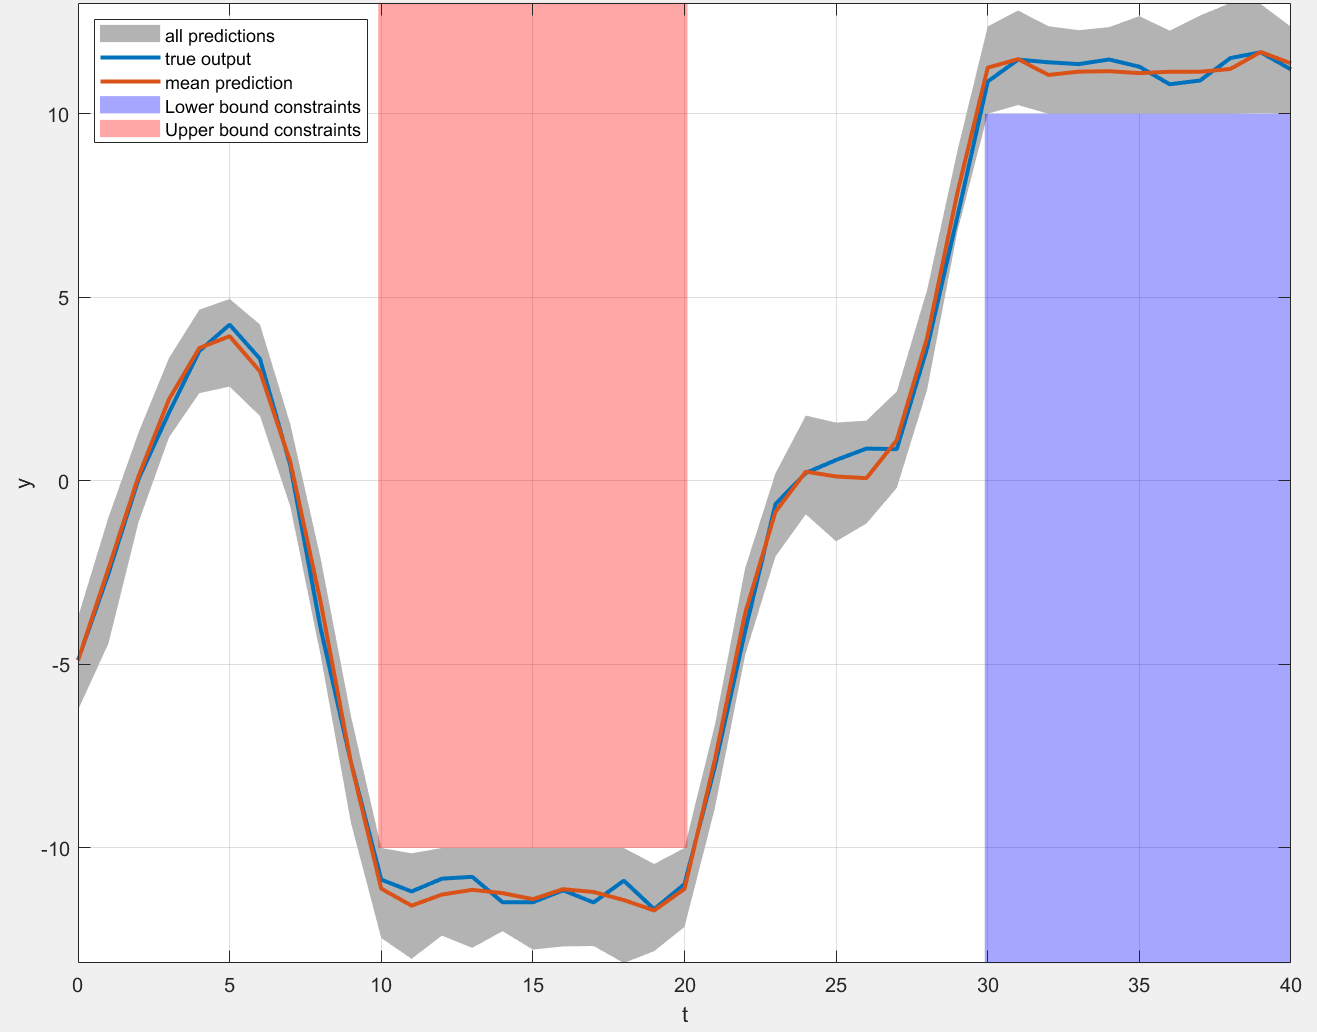
\includegraphics[width=0.4\textwidth] {pics/Scenario_plot.png}
   \label{fig:subfigScenario}
 }
\quad % puts next subfigure right next to the previous subfigure
\subfigure[Kernel Approach]{
   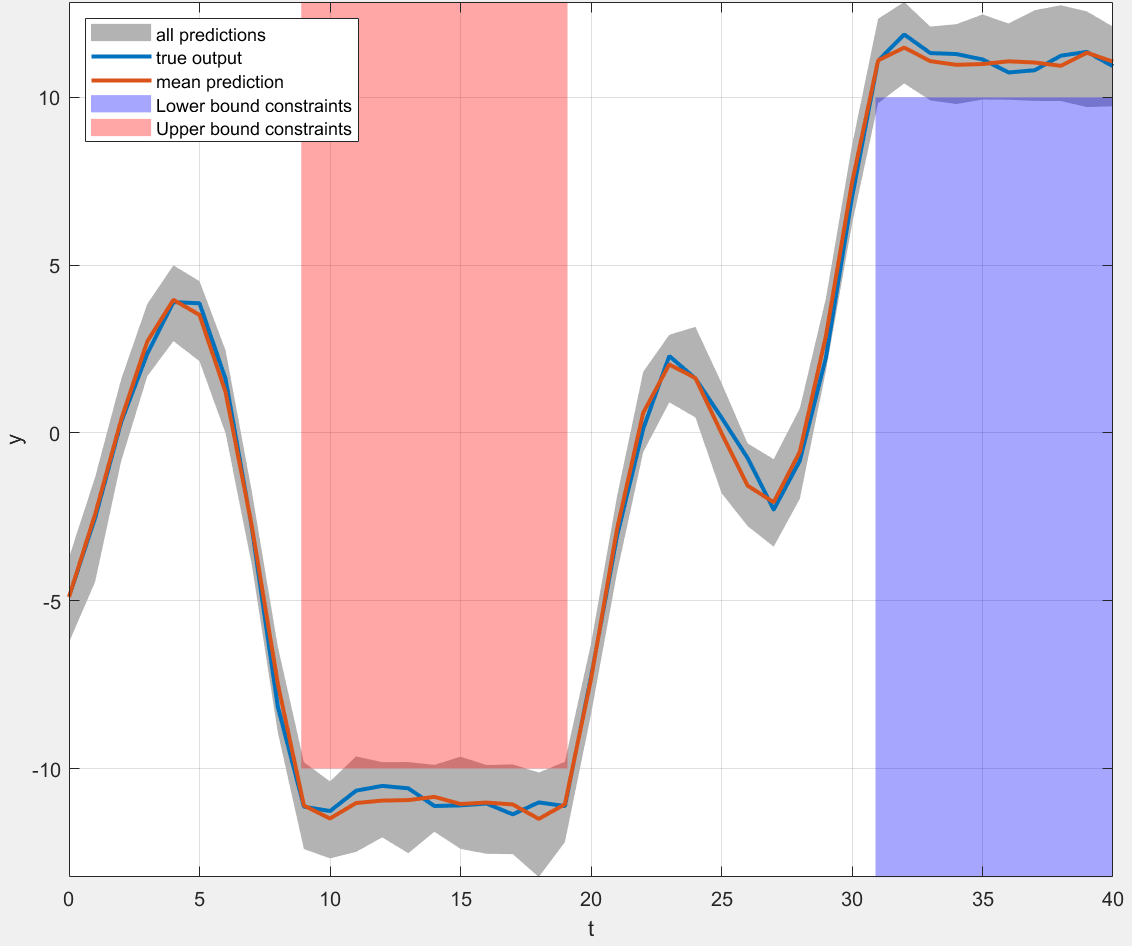
\includegraphics[width=0.4\textwidth] {pics/Kernel_plot.png}
   \label{fig:subfigKernel}
 }
\caption{Example of the optimal control with known basis functions for scenario approach (left) and kernel approach (right). The red and blue area show the output constraints. The gray area encompasses the 200 scenarios that were used in the optimization with the orange line being the average. The blue line is one realization the true output.}
\label{ScenarioKernelComparison}
\end{figure}

The figure includes the two plots for the scenario and kernel approach and shows the output $y$ of their respective OCPs over the time $t = 0, ..., H$. The graphs show the area that the trajectories of all $K = 200$ scenarios generate on top of the mean and true output. Where the two graphs differ however is to what extend the solutions fulfill the constraints. By its definition, the scenario approach requires all scenarios to fulfill the constraints which can be seen in the solution. While the gray area touches the min and max constraints in several places, it never violates the constraints. The kernel approach on the other hand has a risk factor $\alpha$ built in which allows for a number of scenarios to violate the constraints as long a sufficient number satisfies them. This can be seen in the constraint still being met by the majority of the scenarios and only the trajectory of a small number of scenarios actively overlapping with the marked area. As a result, a solution with a lower cost was found in exchange for an increased risk of the true output violating one or more of the constraints.




\section{Robustness} \label{performance guarantees}

The biggest advantage that this kernel approximation proves compared to the scenario approach is the adjustable risk factor. As described in Sec. \ref{Sec:CCOKernel}, this method includes a parameter $\alpha \in [0, 1]$ which can be chosen depending on how accurate the final solution is supposed to be. 

In this section, this parameter is tested by running the same problem setup as was used in Sec. \ref{optimal control} for different values of $\alpha$ as well as an increasing number of samples $N$ and testing how well the solution holds up for future scenarios.

Similar to Sec. \ref{optimal control}, $N = 200$ scenarios are generated with Algorithm \ref{alg:PGibbs}. From this set of 200 scenarios, a small subset is then taken and used to formulate several OCPs as was already described in Sec. \ref{optimal control}. The OCPs are then solved and the resulting optimal input $\boldsymbol{u}_{0:H}$ is then used on $N = 2000$ more independant scenarios from the same system to test how well this solution holds up. For each of the 2000 scenarios, the output is calculated and compared to the constraints that were used in the OCP to check whether or not they are fulfilled. This process is then repeated over and over for a slightly larger subset of scenarios until finally the full set of $N = 200$ scenarios is used.

\begin{figure}[htb]
\centering
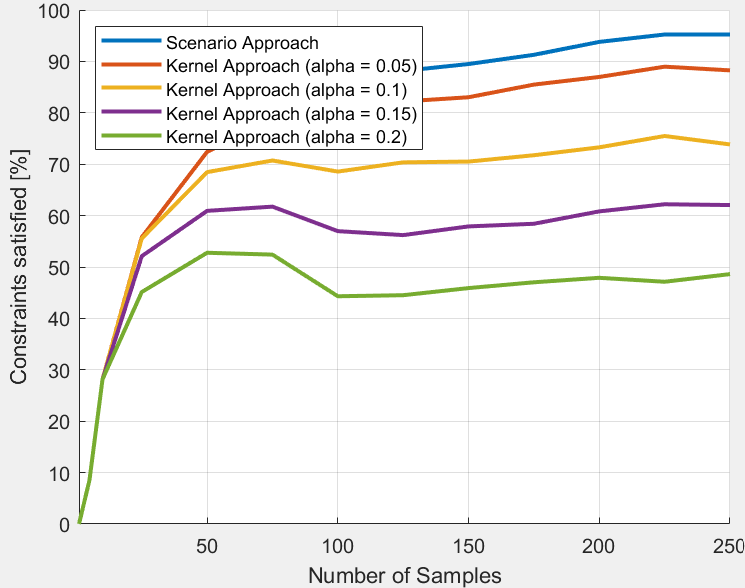
\includegraphics[width=0.7\textwidth]{pics/robustness_plot.png}
\caption{Estimated percentage of scenarios where $u_{0:H}$ is a viable solution. The blue line shows the result of the scenario approach while the other lines are for the Kernel approach with various values of $\alpha$}
\label{fig:robustness_plot}
\end{figure}

In Fig. \ref{fig:robustness_plot} the results of this simulation are shown. The percentage of scenarios that fulfill the constraints is plotted over the number of samples used in the initial optimization which range from $N = 1$ to 200. The various $\alpha$ values are shown as separate lines. Initially, all five plots show very similar results. This can be explained by the fact that at such a low number of scenarios cannot accurately represent the distribution and at this point all cases are still in the process of improving their accuracy. As the number of scenarios is increased, the approximation of the distribution becomes better as well and the solution of the OCP now represents a larger number of the distribution. 

After around 10 scenarios, the plots start diverging for the first time. While the scenario approach and the plots with smaller $\alpha$ values are very similar, the lines that represent larger $\alpha$ values are starting to display worse percentage of cases that satisfy the constraints. This trend continues as the number of scenarios used in the optimization keeps increasing. While the scenario approach keeps increasing, the Kernel approach seems to converge to a significantly lower level of robustness based on the selection of the parameter $\alpha$. This shows that through $\alpha$ we are able to control how distributionally robust the solution is.

 

\section{Computation Time} \label{computation time}

While the previous sections focused on comparing the results of the Scenario approach to the kernel approach, the runtime of both methods is another important factor that needs to be considered when choosing which algorithm is best suited for a specific problem. As such, Fig. \ref{fig:runtime_plot} shows the runtime of both scenario approach and kernel approach over the number of scenarios that are used to formulate the OCPs. The parameters and constraints are chosen the same as in Sec. \ref{optimal control}. When looking at the figure, it quickly becomes apparent that while both curves start around the same level, the kernel approach runtime increases significantly faster and with more of a curvature than the scenario approach. By the end of the plot, the kernel approach already takes about 5 times as long as the scenario approach. This shows that at least when it comes to finding a solution quickly, the Scenario approach is still the better choice.

\begin{figure}[htb]
\centering
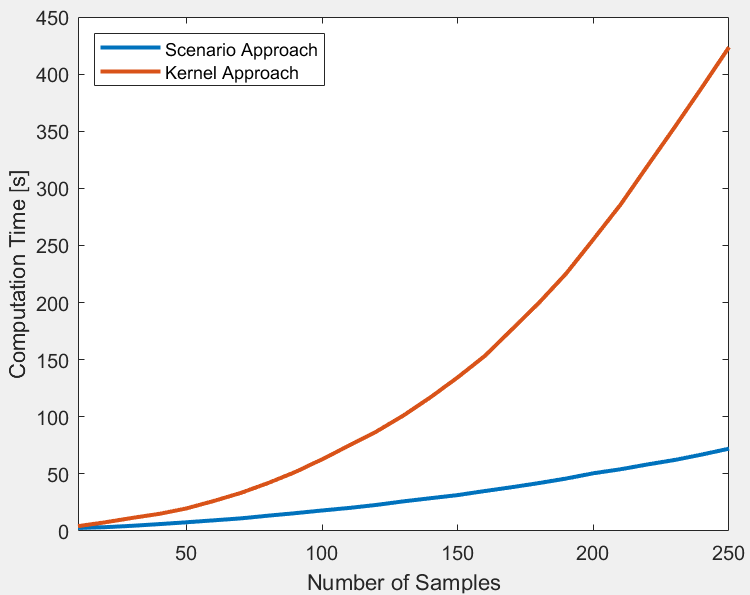
\includegraphics[width=0.6\textwidth]{pics/computationtime_plot.png}
\caption{Runtime over number of scenarios $N$ for scenario and kernel approach}
\label{fig:runtime_plot}
\end{figure}
